% \title{The Soft Massive Spring}
% \author{An Introduction to Physics through Experiments}
% \date{}
% \maketitle

\chapter{The Soft Massive Spring}

\section*{Objectives}

\begin{enumerate}
\item To determine the spring constant and the mass correction factor for the given soft massive
spring by static (equilibrium extension) method.
\item To determine the spring constant and the mass correction factor for the given soft massive
spring by dynamic (spring mass oscillations) method.
\item To determine the frequency of oscillations of the spring with one end fixed and the other
end free i.e. zero mass attached.
\item To study the longitudinal stationary waves and to determine the fundamental frequency of
oscillations of the spring with both the ends fixed.
\end{enumerate}

\section*{Introduction}

Springs are familiar objects with many everyday applications ranging from retractable ballpoint pens, to weighing scales and metro handles. Let us consider an ideal spring: such a spring has an equilibrium length -- that is, a length when no external force is applied -- and resists any change to this length through a restoring force.

%\todo[inline]{Diagram showing forces and springs.}

\begin{figure}[!htb]
    \centering
    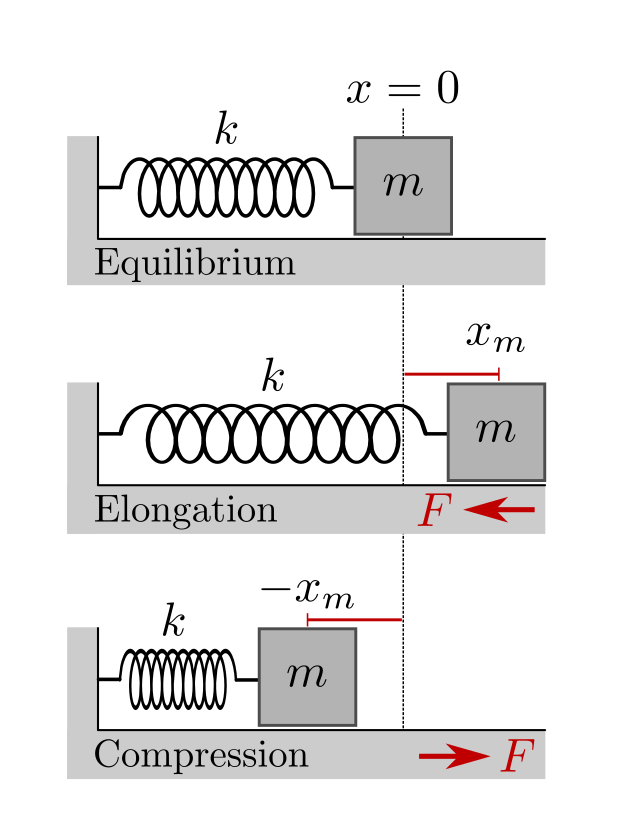
\includegraphics[width=0.4\textwidth]{figs/springForce.png}
    \caption{The restoring force experienced by the mass due to the spring is proportional to the amount the spring is stretched from its equilibrium position.}
    \label{fig:springForces}
\end{figure}

In such ideal springs, the force required to stretch (or compress) is assumed to be proportional to the amount which the spring is stretched (with compression being negative stretching). When one end is fixed, then this stretch is just the displacement of the free end. From now on we will assume that one end is fixed (which implies that we must use the formulas carefully when both ends are free). This tells us that the restoring force i.e.\ $F \propto x$. By defining a constant of proportionality $k$, known as the spring constant, we can write down \textit{Hooke's Law}:

\begin{equation}
    F = - k x,
    \label{hooke}
\end{equation}

where the negative sign shows that the force is in the direction opposite to the displacement of the end, i.e.\ it is a restoring force: when the spring is stretched, this force tends to compress it, and vice versa. Experiment reveals that for relatively small displacements, almost all \textit{real} springs obey Equation (\ref{hooke}).

Let us assume that the spring is placed horizontally on a frictionless surface and attached to a wall on one end and an object of some mass $M$ on the other, which we can pull or push. If we displace the object by some $x$ and let go, it will experience a restoring force due to the spring, which will change as the object begins moving. Combining Newton's Second Law and Equation (\ref{hooke}) we can see that the acceleration of the object is given by

\begin{equation}
\begin{aligned}
    a &= \frac{F}{M} \\
    \dv[2]{x}{t}&=-\frac{k}{M} x
\end{aligned}
\label{diffEqnSimpleSpring}
\end{equation}

where we have chosen $x = 0$ as the equilibrium position of the mass (in which the spring has its unstretched, or equilibrium, length).

%\todo[inline]{Diagram showing horizontal oscillations.}

It is not difficult to see that any function whose second derivative is itself (times a negative constant) is a solution to the differential equation above. Both $\sin (\omega t)$ and $\cos (\omega t)$ are such functions. From the theory of differential equations, we know that the general solution to this differential equation is a linear combination of two linearly independent solutions. Thus we can write

\begin{equation*}
    x(t) = A \sin(\omega t) + B \cos(\omega t),
\end{equation*}

where $\omega$ -- known as the frequency of vibration -- must be equal to $\sqrt{k/M}$ for the left and right sides to match, and $A$ and $B$ are constants determined by the initial conditions (initial position and initial velocity). Observing the solution above, it should be clear to you (since $\sin$ and $\cos$ are periodic functions) that there must be some time $T$ after which $x(t)$ comes back to itself, i.e.\ $x(t+T) = x(t)$. The motion is thus periodic, with period equal to that of the sinusoidal functions $\sin(\omega t)$ and $\cos(\omega t)$, which is

\begin{equation}
    T = \frac{2 \pi}{\omega} = 2\pi \sqrt{\frac{M}{k}}.
    \label{masslessTime}
\end{equation}

The mass thus oscillates about its equilibrium position with a time period $T$ that is -- at least for small amplitudes -- independent of amplitude.

%\todo[inline]{Diagram showing twice the mass and twice the displacement under gravity.}

\begin{figure}[!htb]
    \centering
    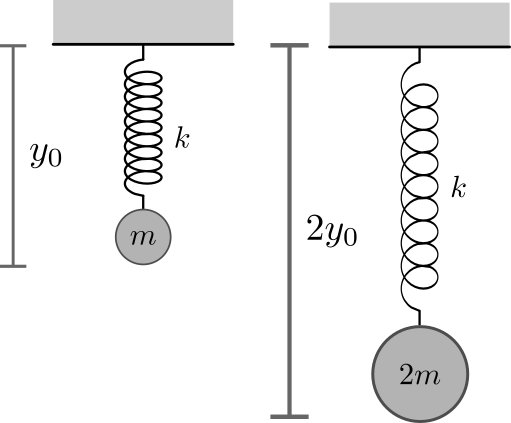
\includegraphics[width=0.3\textwidth]{figs/springMassVertical.png}
    \caption{Hanging vertically, if a mass $m$ causes the spring to extend to $y_0$, a mass of $2m$ will cause the same spring to extend to $2 y_0$.}
    \label{fig:springMassVertical}
\end{figure}


We could now imagine hanging the spring and mass vertically. While the spring is assumed to be massless (as it is ideal), the massive object experiences a downward force due to gravity of $Mg$. At static equilibrium, the spring would have displaced enough to balance this force. Thus,

\begin{equation}
    y_0 = \frac{Mg}{k}.
    \label{masslessExt}
\end{equation}

We could similarly gently displace this spring vertically about this position, and we would again see oscillations, only this time the oscillations will be about the point $y_0$, which is the new equilibrium point.

\begin{figure}[!htb]
    \centering
    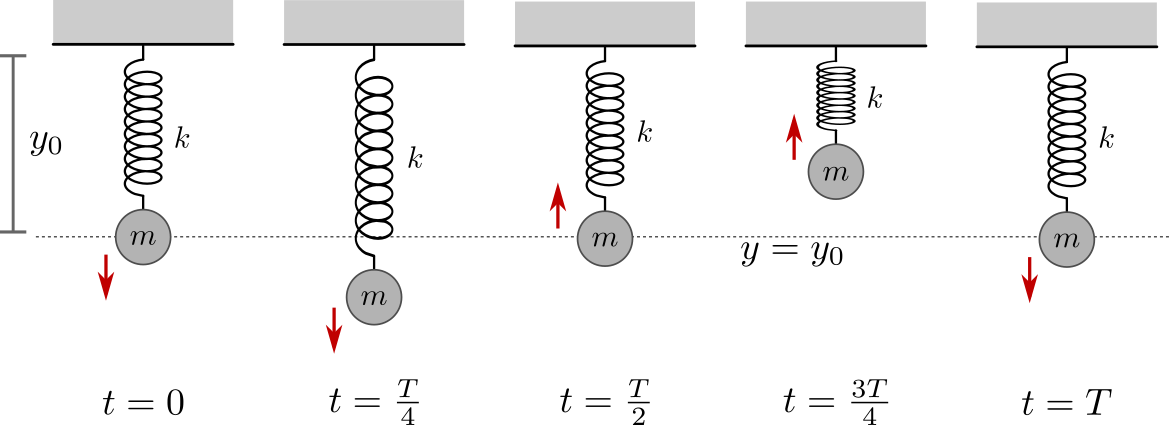
\includegraphics[width=\textwidth]{figs/springOscillations.png}
    \caption{If the vertically hanging spring is displaced slightly, it will begin to oscillate with a time period $T$ about the new equilibrium point $y_0$, as shown.}
    \label{fig:springOscillations}
\end{figure}


\begin{question}
\paragraph{Question:} Write out Newton's Law as a differential equation in this case (i.e.\ when gravity is included). Show that it can be written as:

\begin{equation*}
    \dv[2]{y}{t} = -\omega^2 (y - y_0) 
\end{equation*}

\paragraph{Question:} By making a suitable substitution and comparing it with Equation (\ref{diffEqnSimpleSpring}), show that the solutions have the same form in a shifted variable.

\paragraph{Question:} Show that the time period $T$ is the same as in the preceding case (of ``static'' equilibrium).
\end{question}


\subsection*{Massive springs}

So far, we have assumed our spring to be ``massless'', in that its mass may be neglected. Whether or not this is a reasonable assumption does not depend on the spring alone, but on external factors. 

On inspection, it should be clear to you that the top and the bottom of a spring hung vertically do not experience the same downward or restoring forces, even at static equilibrium.\footnote{In general, a spring is not a ``rigid'' body.} If this ``droop'' (caused by the mass of he spring) is negligible compared to the stretch caused by external masses, then the spring may be effectively considered as massless. Thus it depends roughly on the ratio of the masses.


\subsubsection*{The static case}

Let us consider a point very close to the top of the spring: it will experience a (small) restoring force from the small amount of spring above it, and a much larger downward force from the mass of spring under it. Similarly, consider a point very close to the free end of the spring: it will experience a larger restoring force (as there is more ``spring'' above it) than downward gravitational force as there is very little mass under it. As a result, the spring does not stretch uniformly; the coils near the top are further separated than those near the bottom. We would thus expect some form of ``correction factor'' to the mass term in Equation (\ref{masslessExt}).

Consider a spring with some mass $m_s$. Let $L_0$ be the length of the spring when it is kept horizontally with no forces extending it, and $L_M$ be the length of spring when it is hung vertically with a mass $M$ attached to its lower end. We can define the ``equilibrium extension'' $S_M$ as

\begin{equation}
S_M = L_M - L_0.
\end{equation}

It is possible to solve the problem theoretically and show that the massive spring acts effectively like an ideal spring with a mass $m_s/2$ attached to its end. In other words, if a massive spring is hung vertically, and an ideal spring with mass $m_s/2$ is attached to its end, they will both extend to the same distance.

Thus, Equation (\ref{masslessExt}) is modified to

\begin{equation}
S_M = \left( M + \frac{m_s}{2} \right)\left(\frac{g}{k} \right)
\label{Sm}
\end{equation}

where the factor $m_s/2$ is known as the \textbf{static} mass correction factor.


\subsubsection*{The dynamic case}

Consider now the case of an ideal spring oscillating with a mass attached at its end. The oscillating mass $M$ will have a kinetic energy 

\begin{equation*}
    K_\text{mass} = \frac{1}{2} M v^2
\end{equation*}

However, if the spring itself is massive, since different parts of it move at different velocities, it will also have some kinetic energy associated with it. To find the total kinetic energy of the spring, one could imagine an infinitesimal mass element on the spring moving at some velocity and integrate its contribution to the kinetic energy to get the total energy:\footnote{Though this is slightly advanced, it is not too difficult to do at your level. We urge you to attempt to show this theoretically.}

\begin{equation}
    K_\text{spring} = \frac{1}{6} m_s v^2
\end{equation}

\begin{imp}
This also explains why the spring oscillates even when it has no external mass attached.
\end{imp}

\begin{question}
\paragraph{Question:} Show, from the earlier expressions for kinetic energy, that the spring behaves like an ideal spring with a mass of $m_s/3$ attached to it.
\end{question}

Thus, when an external mass $M$ is attached to the spring, it behaves as if it is effectively an ideal spring with a mass $M+ m_s/3$ attached to its end. Thus, Equation (\ref{masslessTime}) will need to be modified.

The resulting time period $T$ for the oscillations of a massive spring is given by 

\begin{equation}
T = 2\pi \sqrt{\cfrac{\left(M + \cfrac{m_s}{3}\right)}{k}}.
\label{Tm}
\end{equation}

The factor $m_s/3$ is the \textbf{dynamic} mass correction factor. 

\begin{imp}
Note that this factor is different from the mass correction factor in the previous (static) case. The reason for this difference is that they arise from two different processes. In the first case, the effective mass comes from the fact that the different mass-elements comprising the spring experience different forces, which affects the effective \textit{extension}. In the dynamic case where these different mass-elements are \textit{moving}, the term $m_s/3$ comes from the fact that they have different velocities, which affects the effective \textit{kinetic energy}.

%\todo[inline]{Could still use some work.}
\end{imp}

\begin{question}
\paragraph{Question:} Show that if the mass $M$ that is attached is too large compared to $m_s$, Equations (\ref{Sm}) and (\ref{Tm}) give the same results as for an ideal spring. 
\end{question}


When no additional mass is attached to the spring (i.e.\ $M=0$), we can define a corresponding frequency for the massive spring  

\begin{equation}
    f_0 = \frac{1}{T} = \frac{1}{2\pi} \sqrt{\frac{3k}{m_s}}.
\end{equation}


\subsubsection*{Standing waves on a massive spring}

If we stretch the spring between two fixed points, it can be considered as a system with a uniform mass density (say, number of rungs per centimetre). When vibrated with some periodic forcing, this system has its own natural frequencies, very much like sound waves in a hollow pipe closed at both ends.\footnote{The pipe being ``closed'' implies that the amplitude of the waves at both ends is zero. In this case, the top end of the spring is fixed, and the bottom end moves at an amplitude so small compared to the length of the spring, that it can effectively be considered to be fixed.}

\begin{figure}[!htb]
    \centering
    \begin{subfigure}[b]{0.5\textwidth}
        \centering
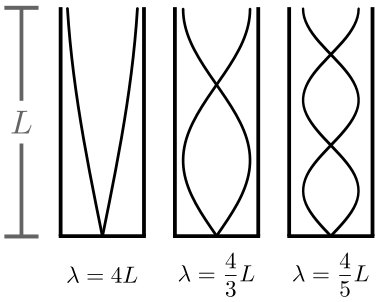
\includegraphics[width=0.8\textwidth]{figs/wavesInAHalfOpenPipe.png}
                \caption{Waves on a pipe with one closed and one open end.}
                \label{fig:wavesInAHalfOpenPipe}
        \end{subfigure}\hfill
        \begin{subfigure}[b]{0.5\textwidth}
        \centering
                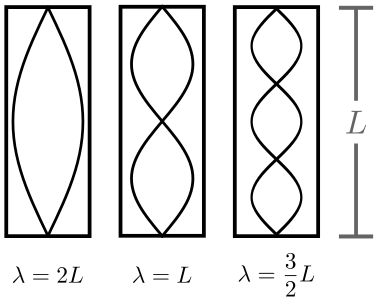
\includegraphics[width=0.8\textwidth]{figs/wavesInAClosedPipe.png}
                \caption{Waves on a pipe with both ends closed.}
                \label{fig:wavesInAClosedPipe}
        \end{subfigure}
    \caption{Variation of amplitude in an air column: Sound waves are characterised by a series of alternate compressions and rarefactions. When an end is closed, the air particles there do not move, and thus that point is a node. Conversely, when the end is open, the particles have the maximum amplitude, and so that point is an antinode.}
    \label{fig:wavesInAPipe}
\end{figure}


When this system is vibrated at one of these ``natural'' frequencies, standing (longitudinal) waves are seen to form, with clear nodes -- i.e.\ points on the spring that remain completely stationary. Two important points can be noticed about the nodes in this case:

\begin{enumerate}[label=(\alph*)]
    \item They divide the length of the spring into equal parts.
    \item They increase by 1 as you move from one natural frequency to the next.
\end{enumerate}

\begin{question}
\paragraph{Question:} Drawing out a diagram like Figure (\ref{fig:wavesInAPipe}), show that the wavelength of a wave with $n$ nodes is given by

\begin{equation}
    \lambda_n = \left(\frac{2}{n+1}\right) L , \quad \quad n=0,1,2\hdots
\end{equation}
where $L$ is the length of the column and $n$ the number of nodes (excluding the fixed endpoints).
\end{question}


We know that waves satisfy the following equation that relates their wavelengths and frequencies, 

\begin{equation}
    v = f_n \lambda_n
\end{equation}

where $v$ is the velocity of the wave. As this is a constant for a configuration, it follows that 

\begin{equation}
\begin{aligned}
f_n = \frac{v}{\lambda_n} &= \frac{v (n+1)}{2L}\\
f_1 = \frac{v}{2L}, \quad f_2 = \frac{v}{L},\quad &\hdots,\quad f_n = n f_1.
\end{aligned}
\end{equation}



\section*{Experimental Setup}

\subsection*{Apparatus}

\begin{enumerate}[label=\arabic*)]
\itemsep0em
\item A set of soft massive springs
\item A long and heavy retort stand with a clamp at the top end 
\item A set of masses with hooks
\item A signal generator (\textit{Equip-tronics QT-210})
\item A dual output power amplifier with the connecting cords
\item A mechanical vibrator
\item A digital multimeter (\textit{Victor VC97})
\item A digital stopwatch (\textit{Racer})
\item Measuring tapes
\item A set of measuring scales (1.0 m, 0.6 m and 0.3 m)
\end{enumerate}

\subsection*{Description}

\begin{description}

\item[Digital Multimeter (\textit{Victor VC97})]

A multimeter is an instrument used to measure multiple parameters like voltage, current, and resistance. You will be using the multimeter to measure the frequency of the signal. You will have to use input sockets marked COM, V/$\Omega$ to do this. Note that the two input sockets marked mA and 10A are for the current measurement. You will not be using those. Connect the banana cables to COM and V/$\Omega$, and select the Hz setting on the multimeter. 

\item[Signal Generator]

A signal generator is used to generate simple repetitive waveforms in the form of an alternating electrical wave. Typically, it will produce simple waveforms like sine, square, and triangular waves, and will allow you to adjust the frequency and amplitude of these signals. The instrument given to you generates sine, sawtooth, and square waveforms. The output may be taken from the respective output sockets through banana cables. The frequency can be adjusted by turning the frequency dial and turning the Range knob to the appropriate multiplier. For example, turning the dial to 3 and selecting the 100X setting in the range knob would provide an output waveform with a frequency of 300Hz. Similarly the amplitude knob varies the amplitude of the output waveform.

\begin{tip}
The DC Offset button makes the signal oscillate about a constant non-zero DC voltage (instead of zero). Normally, this shouldn't affect the working of the setup. However, when a multimeter is connected to it to measure frequency, it will not be able to do so, as it is calibrated to measure signals alternating about zero.
\end{tip}

\item[Mechanical Vibrator]

The mechanical vibrator converts the electrical signals from the signal generator into mechanical vibrations, similar to how a speaker works. When using the spring as a uniform mass distribution, it should be clamped at one end of the stand, and its lower end should be clamped to the crocodile clip fixed on the vibrator. This end will be subjected to an up and down harmonic motion which will constitute the ``forcing'' of the spring. It must be ensured that the amplitude of this motion is small enough so that these ends could be considered to be fixed.


\item[Power Amplifier]

The Power Amplifier is used to amplify the signals from the signal generator before it is sent to the mechanical vibrator. The reason for this is two-fold: the signal itself is not sufficiently strong, and even if it were, there is a risk that a signal with a large amplitude could damage the mechanical vibrator. In order to prevent this, the amplifier has been equipped with two fuses to protect the vibrator.

\end{description}





\subsection*{Precautions}

\begin{itemize}
\item Don't overload the spring or you will stretch it beyond its elastic limit and damage it.
\item Keep the amplitude of oscillations of the spring-mass system just sufficient to get the required number of oscillations.
\item The amplitude of vibrations should be carefully adjusted to the required level using the amplitude knob of the signal generator so as to not blow the fuse in the power amplifier. The brighter and more frequently the indicator LEDs flash, the closer the fuse is to blowing.
\end{itemize}

\section*{Procedure}

\subsection*{Part A}

In this part, you will use the static method to determine the spring constant of a massive spring, by measuring the equilibrium extension of a given spring for different attached masses.

\begin{enumerate}
\item Measure the length $L_0$ of the spring keeping it horizontal on a table in an unstretched (all the coils touching each other) position.
\item Hang the spring to the clamp fixed to the top end of the retort stand. The spring extends under its own weight.
\item Take appropriate masses and attach them to the lower end of the spring. 
\item Measure the length $L_M$ of the spring in each case. (For better results you may repeat
each measurement two or three times.) Thus determine the equilibrium extension $S_M$ for each value of mass attached.
\item Plot an appropriate graph and determine the spring constant $k$ and mass of the spring $m_s$.
\item Weigh the spring and compare its mass $m_s$ with the one obtained from the graph experimentally.
\end{enumerate}

\begin{question}
\paragraph{Question:} State and justify the selection of variables plotted on the $x$ and $y$ axes. Explain the observed behaviour and interpret the $x$ and $y$ intercepts.
\end{question}


\subsection*{Part B}

In this part you will use the dynamic method to find the time period of a massive spring with different masses attached. The frequency of oscillations of the spring with the upper end fixed and the lower end free (i.e. with no attached mass) will be determined graphically through extrapolation.

\begin{enumerate}
\item Keep the spring clamped to the retort stand.

\item Try to set the spring into oscillations without any mass attached, you will observe that the spring oscillates under the influence of its own weight.

\item Attach different masses to the lower end of the spring and measure the time period of oscillations of the spring mass system for each value of the mass attached. You may measure the time for a number of oscillations to determine the average time period.

\item Perform the necessary data analysis and determine spring constant $k$ and the mass of the spring $m_s$ using the above data. Compare these values to those obtained in the Part A.

\item Also determine frequency $f_0$ for zero mass attached to the spring from the graph.

\end{enumerate}


\subsection*{Part C}

In this part, you will use a mechanical vibrator to force oscillations on the spring and excite its different normal modes of vibrations. Thus the longitudinal stationary waves will be set up on the spring, whose frequencies will be measured. The fundamental frequency $f_1$ in this case will be compared with $f_0$ obtained in \textbf{Part B}.

\begin{enumerate}
\item Keep the spring clamped to the long retort stand.

\item Clamp the lower end of the spring to the crocodile clip attached to the vibrator.

\item Connect the output of the signal generator to the input of the mechanical vibrator through the power amplifier, using a BNC cable.

\item Connect a the multimeter to the signal generator and set it to measure frequency.

\begin{tip}
While it might seem sensible to connect the multimeter to the mechanical vibrator, it is found that the amplification of the signal leads to a problem in detecting its frequency. Thus, it is better to connect it directly to the signal generator.
\end{tip}

\item Starting from zero, slowly increase the frequency of the sinusoidal signal generated by the signal generator. At some particular frequency you will observe the formation of nodes: points on the spring which appear clearly visible as they are not moving.

\item Increase the frequency further and observe higher harmonics identifying them on the basis of the number of loops you can see between the fixed ends. (If you see $n$ nodes -- or fixed points -- between the endpoints, there are $n+1$ loops.)

\item Plot a graph of frequency for different number of loops versus the number of loops. Determine this fundamental frequency $f_1$ from the slope of this graph.

\item Compare this fundamental frequency $f_1$ with the frequency $f_0$ of the spring mass
system with one end fixed and the zero mass attached (as determined in Part B) and
show that $$f_0 = \frac{f_1}{2}$$
\end{enumerate}

\begin{question}
\paragraph{Question:} Can you think of why the two frequencies should be related by a factor of two? (You may use the analogy between the spring and an air column.)
\end{question}


\section*{References}

\begin{enumerate}
\itemsep0em
\item J. Christensen, \textit{Am. J. Phys}, 2004, 72(6), 818-828.

\item T. C. Heard, N. D. Newby Jr, Behavior of a Soft Spring, \textit{Am. J. Phys}, 45 (11), 1977,
pp. 1102-1106. 

\item H. C. Pradhan, B. N. Meera, Oscillations of a Spring With Non-negligible Mass, \textit{Physics Education (India)}, 13, 1996, pp. 189-193.

\item B. N. Meera, H. C. Pradhan, Experimental Study of Oscillations of a Spring with Mass Correction, \textit{Physics Education (India)}, 13, 1996, pp. 248-255.

\item Rajesh B. Khaparde, B. N. Meera, H. C. Pradhan, Study of Stationary Longitudinal Oscillations on a Soft Spring, \textit{Physics Education (India)}, 14, 1997, pp. 130-19. 

\item H. J. Pain, \textit{The Physics of Vibrations and Waves}, 2nd Ed, John Wiley \& Sons, Ltd., 1981.

\item D. Halliday, R. Resnick, J. Walker, \textit{Fundamentals of Physics}, 5th Ed, John Wiley \& Sons, Inc., 1997.

\item K. Rama Reddy, S. B. Badami, V. Balasubramanian, \textit{Oscillations and Waves}, University
Press, Hyderabad, 1994.
\end{enumerate}

\newpage